\documentclass[10pt]{beamer}\usepackage[]{graphicx}\usepackage[]{color}
%% maxwidth is the original width if it is less than linewidth
%% otherwise use linewidth (to make sure the graphics do not exceed the margin)
\makeatletter
\def\maxwidth{ %
  \ifdim\Gin@nat@width>\linewidth
    \linewidth
  \else
    \Gin@nat@width
  \fi
}
\makeatother

\definecolor{fgcolor}{rgb}{0.345, 0.345, 0.345}
\newcommand{\hlnum}[1]{\textcolor[rgb]{0.686,0.059,0.569}{#1}}%
\newcommand{\hlstr}[1]{\textcolor[rgb]{0.192,0.494,0.8}{#1}}%
\newcommand{\hlcom}[1]{\textcolor[rgb]{0.678,0.584,0.686}{\textit{#1}}}%
\newcommand{\hlopt}[1]{\textcolor[rgb]{0,0,0}{#1}}%
\newcommand{\hlstd}[1]{\textcolor[rgb]{0.345,0.345,0.345}{#1}}%
\newcommand{\hlkwa}[1]{\textcolor[rgb]{0.161,0.373,0.58}{\textbf{#1}}}%
\newcommand{\hlkwb}[1]{\textcolor[rgb]{0.69,0.353,0.396}{#1}}%
\newcommand{\hlkwc}[1]{\textcolor[rgb]{0.333,0.667,0.333}{#1}}%
\newcommand{\hlkwd}[1]{\textcolor[rgb]{0.737,0.353,0.396}{\textbf{#1}}}%
\let\hlipl\hlkwb

\usepackage{framed}
\makeatletter
\newenvironment{kframe}{%
 \def\at@end@of@kframe{}%
 \ifinner\ifhmode%
  \def\at@end@of@kframe{\end{minipage}}%
  \begin{minipage}{\columnwidth}%
 \fi\fi%
 \def\FrameCommand##1{\hskip\@totalleftmargin \hskip-\fboxsep
 \colorbox{shadecolor}{##1}\hskip-\fboxsep
     % There is no \\@totalrightmargin, so:
     \hskip-\linewidth \hskip-\@totalleftmargin \hskip\columnwidth}%
 \MakeFramed {\advance\hsize-\width
   \@totalleftmargin\z@ \linewidth\hsize
   \@setminipage}}%
 {\par\unskip\endMakeFramed%
 \at@end@of@kframe}
\makeatother

\definecolor{shadecolor}{rgb}{.97, .97, .97}
\definecolor{messagecolor}{rgb}{0, 0, 0}
\definecolor{warningcolor}{rgb}{1, 0, 1}
\definecolor{errorcolor}{rgb}{1, 0, 0}
\newenvironment{knitrout}{}{} % an empty environment to be redefined in TeX

\usepackage{alltt}
\usepackage{amsmath}
\usepackage{amssymb}
\usepackage{geometry}
\usepackage{graphicx}
\usepackage{url}
\usepackage{bm}

\makeatletter
\let \@sverbatim \@verbatim
\def \@verbatim {\@sverbatim \verbatimplus}
{\catcode`'=13 \gdef \verbatimplus{\catcode`'=13 \chardef '=13 }} 
\makeatother
\IfFileExists{upquote.sty}{\usepackage{upquote}}{}
\begin{document}
\setlength\parindent{0pt}

% --------------------------------------------
\begin{frame}
\large
Lecture 18: Multiple Logistic Regression\\
%Multiple Logistic Regression\\
STAT 632, Spring 2020\\
\end{frame}

% --------------------------------------------
\begin{frame}{Multiple Logistic Regression}
\begin{itemize}
\item Multiple logistic regression is a method to model a binary response variable, $Y \in \{0,1\}$, using predictor variables $x_1, x_2, \cdots, x_p$.\\
\vspace{10pt}
\item Specifically, the method models $p(\bm{x}) = Pr(Y=1|\bm{x})$, the probability $Y=1$ given predictors $\bm{x} = \begin{pmatrix} x_1 & x_2 & \cdots & x_p \end{pmatrix} '$.  
\end{itemize}
\end{frame}

% --------------------------------------------
\begin{frame}{Multiple Logistic Regression}
Two ways to express multiple logistic regression model:\\
\vspace{20pt}

Probability form:
\begin{align*}
p(\bm{x}) = Pr(Y=1 | \bm{x})
= \frac{e^{\beta_0 + \beta_1 x_1 + \cdots + \beta_p x_p}}{1 + e^{\beta_0 + \beta_1 x_1 + \cdots + \beta_p x_p}}
= \frac{1}{1 + e^{-\beta_0 - \beta_1 x_1 - \cdots - \beta_p x_p}}\\
\end{align*}

Logit form:
\begin{align*}
\log\left( \frac{p(\bm{x})}{1-p(\bm{x})} \right) = \beta_0 + \beta_1 x_1 + \cdots + \beta_p x_p
\end{align*}
\end{frame}

% --------------------------------------------
\begin{frame}{Example: 2016 US Presidential Election}
\begin{itemize}
\item Again, we use the data set called \texttt{Election16} from the \texttt{Stat2Data} library.  The data contain results from the 2016 presidential election and demographic information from all 50 states.
\vspace{10pt}
\item The binary response variable is \texttt{TrumpWin}, whether Trump won the state (1=yes, 0=no).
\vspace{10pt}
\item The predictors are
\begin{itemize}
\item \texttt{HS}: Percent of high school graduates in the state
\item \texttt{BA}: Percent of college graduates in the state
\item \texttt{Adv}: Percent with advanced degrees in the state
\item \texttt{Dem.Rep}:  Percent Democratic - Percent Republican
\item \texttt{Income}: Per capita income in the state
\end{itemize}
\end{itemize}
\end{frame}

% --------------------------------------------
\begin{frame}{Example}
We'll start by considering a multiple logistic regression model for \texttt{TrumpWin}, using two predictors from the data set: \texttt{BA} and \texttt{Dem.Rep}. 
% chage colors trumpwin = red
\begin{figure}
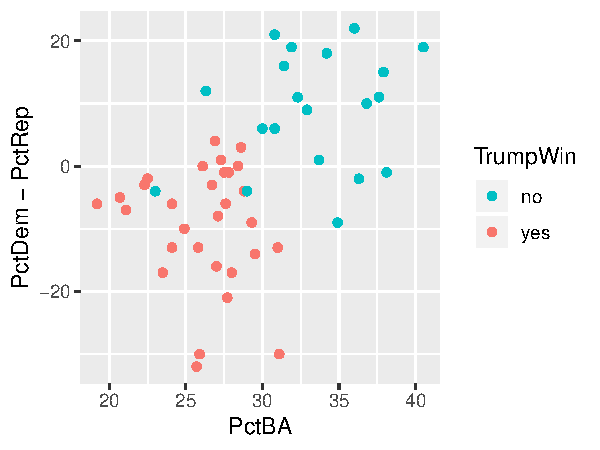
\includegraphics[scale=0.8]{figure/scatter1.pdf}
\end{figure}
\end{frame}

% --------------------------------------------
\begin{frame}[fragile]{Example}
We'll start by considering a multiple logistic regression model for \texttt{TrumpWin}, using two predictors from the data set: \texttt{BA} and \texttt{Dem.Rep}. 
\small
\begin{verbatim}
> glm2 <- glm(TrumpWin ~  BA + Dem.Rep, data=Election16, 
              family=binomial) 
              
> summary(glm2)

Coefficients:
            Estimate Std. Error z value Pr(>|z|)  
(Intercept) 15.34796    6.13130   2.503   0.0123 *
BA          -0.51792    0.21181  -2.445   0.0145 *
Dem.Rep     -0.21406    0.08778  -2.439   0.0147 *

> confint(glm2)
                 2.5 %      97.5 %
(Intercept)  5.7651914 31.36586108
BA          -1.0790415 -0.18972992
Dem.Rep     -0.4357941 -0.07794399
\end{verbatim}
\normalsize
\end{frame}

% --------------------------------------------
\begin{frame}{Example}
\begin{figure}
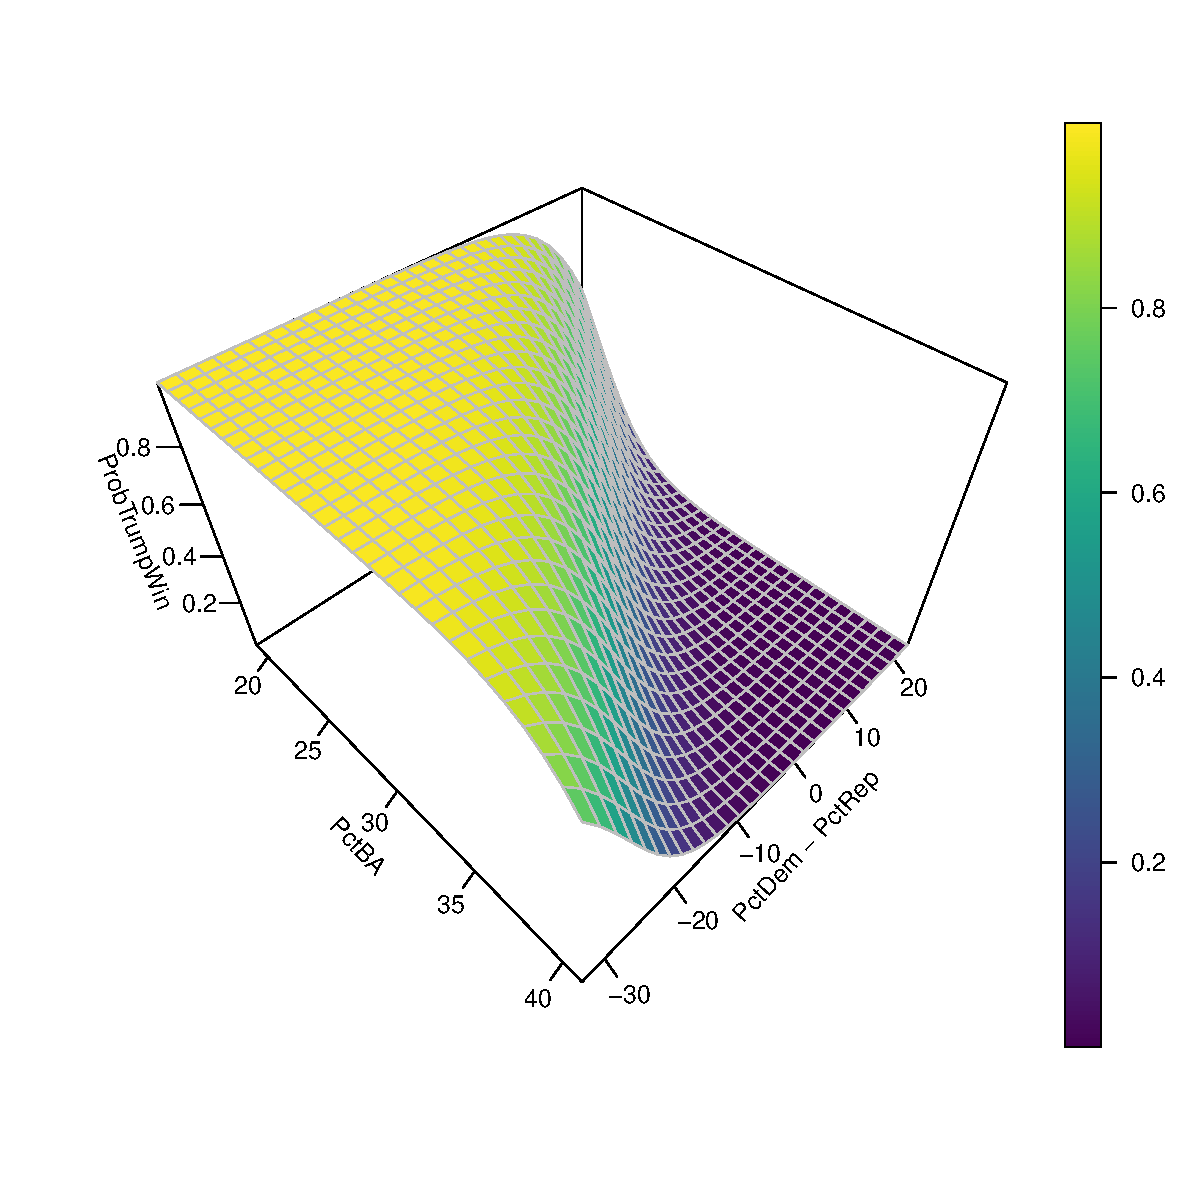
\includegraphics[scale=0.4]{figure/logit3D.pdf}
\end{figure}
\end{frame}

% --------------------------------------------
\begin{frame}[fragile]
\vspace{-2cm}
The code used to create the last plot:
\scriptsize
\begin{verbatim}
> library(plot3D)
> library(viridis)
> glm2 <- glm(TrumpWin ~  BA + Dem.Rep, data=Election16, family=binomial)
> x1vals <- seq(19, 41, len=30)
> x2vals <- seq(-33, 23, len=30)
> grd <- expand.grid(BA = x1vals, Dem.Rep = x2vals)
> preds <- predict(glm2, grd, type="response")
> persp3D(x1vals, x2vals, matrix(preds, 30, 30), col = viridis(200),
          theta=45, phi= 45, ticktype="detailed", expand=0.7, border="grey",
          xlab = "PctBA", ylab = "PctDem - PctRep", zlab = "ProbTrumpWin")
\end{verbatim}
\end{frame}

% --------------------------------------------
\begin{frame}{Example}
The equation for the fitted logistic regression model in probability form is given by:
\begin{align*}
\hat{p}(x_1, x_2) = \frac{e^{\hat{\beta}_0 + \hat{\beta}_1 x_1 + \hat{\beta}_2 x_2}}{1 + e^{\hat{\beta}_0 + \hat{\beta}_1 x_1 + \hat{\beta}_2 x_2}}
= \frac{e^{15.348 - 0.518 x_1 - 0.214 x_2}}{1 + e^{15.348 - 0.518 x_1 - 0.214 x_2}}
\end{align*}
\vspace{10pt}

In California, the \% with a BA is 31.4, and \texttt{Dem.Rep}, the \% Democrat minus the \% Republican, is 16.  So the estimate for the probability that Trump won is   
\begin{align*}
\hat{p}(31.4, 16)
= \frac{e^{15.348 - 0.518(31.4) - 0.214(16)}}{1 + e^{15.348 - 0.518(31.4) - 0.214(16)}} = 
\frac{e^{-4.34}}{1+e^{-4.34}} = 0.0129
\end{align*}
\end{frame}


% --------------------------------------------
\begin{frame}[fragile]{Example}
To make the predictions in R use the \texttt{predict()} function:
\begin{verbatim}
> new_x <- data.frame(BA = 31.4, Dem.Rep = 16)

# prediction for logit
> predict(glm2, newdata=new_x)
        1 
-4.339819 

# prediction for probability
> predict(glm2, newdata=new_x, type="response")
         1 
0.01287107 
\end{verbatim}
\end{frame}

% --------------------------------------------
\begin{frame}{Example}
The line associated with a 0.50 probability of Trump winning is found by setting $\hat{p}(x_1, x_2) = 0.5$, which gives the line $\hat{\beta}_0 + \hat{\beta}_1 x_1 + \hat{\beta}_2 x_2 = 0$.  This is often called the \textbf{decision boundary}.
\begin{figure}
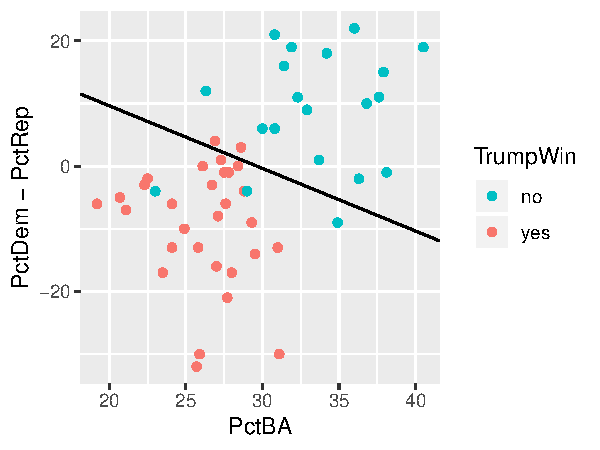
\includegraphics[scale=0.7]{figure/scatter2.pdf}
\end{figure}
\end{frame}

\begin{frame}
\end{frame}

% --------------------------------------------
\begin{frame}{Variable Selection}
For logistic regression modeling, the AIC is defined as
\begin{align*}
\text{AIC} = -2 \log(L(\hat{\bm{\beta}})) + 2K
\end{align*}
where $\log(L(\hat{\bm{\beta}}))$ is the log-likelihood evaluated at the MLEs, $\bm{\hat{\beta}} = \begin{pmatrix} \hat{\beta}_0 & \hat{\beta}_1 & \cdots & \hat{\beta}_p \end{pmatrix}'$, and $K = p+1$ is the number of parameters.
\vspace{10pt}

\begin{itemize}
\item The \emph{smaller} the value for the AIC the better the logistic regression model fits the data.
\vspace{5pt}
\item If we fit several logistic regression models, using the same data set, we would select the model with the smallest AIC value.   
\vspace{5pt}
\item The goodness-of-fit of the logistic regression model is measured by the log-likelihood.  Note that maximizing the log-likelihood is the same as minimizing the negative log-likelihood.    
\end{itemize}
\end{frame}

% --------------------------------------------
\begin{frame}{Variable Selection: Example}
Consider all 8 possible logistic regression models for \texttt{TrumpWin}, using \texttt{BA}, \texttt{Dem.Rep}, and \texttt{Income} as potential predictors.
\begin{table}
\begin{tabular}{l|l}
Predictor Variables & AIC\\
\hline
Null model (intercept only) & 69.30\\
\texttt{BA} & 38.43\\
\texttt{Dem.Rep} & 37.60\\
\texttt{Income} & 49.92\\
\texttt{BA}, \texttt{Dem.Rep} & 27.08\\
\texttt{BA}, \texttt{Income} & 40.12\\
\texttt{Dem.Rep}, \texttt{Income} & \textbf{26.79}\\
\texttt{BA}, \texttt{Dem.Rep}, \texttt{Income} & 27.62\\
\end{tabular}
\end{table}
\end{frame}

% --------------------------------------------
\begin{frame}[fragile]{Variable Selection: Example}
Here is the code used for the previous table:
\scriptsize
\begin{verbatim}
> glm0 <- glm(TrumpWin ~ 1, data=Election16, family=binomial)
> glm1_1 <- glm(TrumpWin ~  BA, data=Election16, family=binomial)
> glm1_2 <- glm(TrumpWin ~ Dem.Rep, data=Election16, family=binomial)
> glm1_3 <- glm(TrumpWin ~  Income, data=Election16, family=binomial)
> glm2_1 <- glm(TrumpWin ~ BA + Dem.Rep, data=Election16, family=binomial)
> glm2_2 <- glm(TrumpWin ~ BA + Income, data=Election16, family=binomial)
> glm2_3 <- glm(TrumpWin ~  Dem.Rep + Income, data=Election16, family=binomial) 
> glm3 <- glm(TrumpWin ~ Income + BA + Dem.Rep, data=Election16, family=binomial)
> AIC(glm0, glm1_1, glm1_2, glm1_3, glm2_1, glm2_2, glm2_3, glm3)
       df      AIC
glm0    1 69.30117
glm1_1  2 38.43266
glm1_2  2 37.59612
glm1_3  2 49.92250
glm2_1  3 27.08020
glm2_2  3 40.12465
glm2_3  3 26.79370
glm3    4 27.62363
\end{verbatim}
\end{frame}

% --------------------------------------------
\begin{frame}[fragile]{Variable Selection: Example}
We can also use the \texttt{step()} function to implement backwards stepwise selection for logistic regression using the AIC.
\small
\begin{verbatim}
> glm5 <- glm(TrumpWin ~ HS + BA + Adv + Dem.Rep + Income, 
                data=Election16, family = binomial)
> glm_sel <- step(glm5)
> summary(glm_sel)
Coefficients:
              Estimate Std. Error z value Pr(>|z|)   
(Intercept)  1.458e+01  5.308e+00   2.747  0.00601 **
Dem.Rep     -3.099e-01  1.135e-01  -2.731  0.00632 **
Income      -2.677e-04  9.866e-05  -2.713  0.00667 **

> AIC(glm5, glm_sel)
        df      AIC
glm5     6 31.55431
glm_sel  3 26.79370
\end{verbatim}
\normalsize
\end{frame}




\end{document}
